\documentclass[12pt]{article}
\usepackage[utf8]{inputenc}
\usepackage{latexsym,amssymb,amsmath} % for \Box, \mathbb, split, etc.
% \usepackage[]{showkeys} % shows label names
\usepackage{cite} % sorts citation numbers appropriately
\usepackage{path}
\usepackage{url}
\usepackage{verbatim}
\usepackage[pdftex]{graphicx}
\usepackage{epstopdf}
\usepackage{mathpazo}
\usepackage{blindtext}
\usepackage{tabularx,ragged2e}
\usepackage{booktabs}
\usepackage{subcaption}

% horizontal margins: 1.0 + 6.5 + 1.0 = 8.5
\setlength{\oddsidemargin}{0.0in}
\setlength{\textwidth}{6.5in}
% vertical margins: 1.0 + 9.0 + 1.0 = 11.0
\setlength{\topmargin}{0.0in}
\setlength{\headheight}{12pt}
\setlength{\headsep}{13pt}
\setlength{\textheight}{625pt}
\setlength{\footskip}{24pt}

\renewcommand{\textfraction}{0.10}
\renewcommand{\topfraction}{0.85}
\renewcommand{\bottomfraction}{0.85}
\renewcommand{\floatpagefraction}{0.90}
\renewcommand{\baselinestretch}{1.2}

\makeatletter
\setlength{\arraycolsep}{2\p@} % make spaces around "=" in eqnarray smaller
\makeatother

% change equation, table, figure numbers to be counted inside a section:
\numberwithin{equation}{section}
\numberwithin{table}{section}
\numberwithin{figure}{section}

% begin of personal macros
\newcommand{\half}{{\textstyle \frac{1}{2}}}
\newcommand{\eps}{\varepsilon}
\newcommand{\myth}{\vartheta}
\newcommand{\myphi}{\varphi}

\newcommand{\IN}{\mathbb{N}}
\newcommand{\IZ}{\mathbb{Z}}
\newcommand{\IQ}{\mathbb{Q}}
\newcommand{\IR}{\mathbb{R}}
\newcommand{\IC}{\mathbb{C}}
\newcommand{\Real}[1]{\mathrm{Re}\left({#1}\right)}
\newcommand{\Imag}[1]{\mathrm{Im}\left({#1}\right)}

\newcommand{\norm}[2]{\|{#1}\|_{{}_{#2}}}
\newcommand{\abs}[1]{\left|{#1}\right|}
\newcommand{\ip}[2]{\left\langle {#1}, {#2} \right\rangle}
\newcommand{\der}[2]{\frac{\partial {#1}}{\partial {#2}}}
\newcommand{\dder}[2]{\frac{\partial^2 {#1}}{\partial {#2}^2}}

\newcommand{\nn}{\mathbf{n}}
\newcommand{\xx}{\mathbf{x}}
\newcommand{\uu}{\mathbf{u}}

\newcommand{\junk}[1]{{}}

% set two lengths for the includegraphics commands used to import the plots:
\newlength{\fwtwo} \setlength{\fwtwo}{0.45\textwidth}
% end of personal macros
\graphicspath{ {../../../resources/images/vectors/}{../../../resources/images/bits/} }

\begin{document}
%\DeclareGraphicsExtensions{.jpg}

\begin{center}
\textbf{\Large Smart Usage of Context Information for the Analysis, Design, and Generation of Power-Aware Policies for Mobile Sensing Apps} \\[16pt]


\includegraphics[scale=0.08]{cinvestav2.jpg}

\textbf{Technical Report}\\[6pt]
LTI-TR-2014-07 \\[16pt]

\textbf{Student} Rafael Pérez-Torres \\[6pt]
\textbf{Advisors} César Torres Huitzil Phd, Hiram Galeana Zapién Phd.\\[16pt]

Information Technology Laboratory,\\
CINVESTAV Tamaulipas \\[16pt]

%  gobbert@umbc.edu, \url{www.math.umbc.edu/~gobbert}
\end{center}

\abstract{
% The popularity of modern smartphones and mobile sensing apps is a consequence of the mobility and increasing storage, computing and communication features of these devices. 
% Because of this, the smartphone has become a full time companion of user. 
% Nevertheless, the energy consumption in mobile sensing apps represents an open problem in the research that has been addressed from several perspectives since its relevance through all layers of the mobile platform.

% This technical report describes the initial stage of the work thesis focused in solving the energy issue from a software perspective.
% The report describes the advances developed during the first period of the doctoral program, including a description of the problem, and focused in the review of the state of art which presents a preliminary taxonomy of works addressing this problem.
% Also, the review of the method pursued in this research for solving the energy consumption problem is also presented.

This technical report presents the fundamental aspects and advances developed in the work thesis titled \emph{Smart Usage of Context Information for the Analysis, Design, and Generation of Power-Aware Policies for Mobile Sensing Apps} during the first period of the doctoral program.
Most of these advances refer to the state of art research, and include the description of a preliminary taxonomy of works aiming to solve the energy consumption problem by the mobile sensing apps.

Also, the review of the method pursued in this research for solving the energy consumption problem is presented.
}

\subparagraph{Keywords.} Provide five key words or phrases that
describe your topic, methods, and results.

\section{Preamble}
\label{sec:preamble}
This technical report describes the advanced performed during the first period of the doctoral program regarding to the thesis work titled \emph{Smart Usage of Context Information for the Analysis, Design, and Generation of Power-Aware Policies for Mobile Sensing Apps}.

Most of the advances obtained in this first period are related to the state of art research, including the generation of a taxonomy of previous related works.
However, in order to prepare a self-contained document, this report also reviews the scientific context of the research describing elements like motivation, problem statement, hypothesis, objectives and contributions.

This technical report is structured as follows.
Initially, the report reviews the problem of the energy consumption in mobile sensing apps, including the problem statement, hypothesis, objectives and contributions pursued by this research work starting from Subsection \ref{sub:introduction}.
Next, a brief description of the core elements of the theoretical framework is presented in Section \ref{sec:theoretical_framework}; this description is useful for a better understanding of the elements involved in the problem.

The Section \ref{sec:state_of_art} comprehends most of the advances developed during this initial period. 
Inside this, the Subsection \ref{sub:approaches_for_addressing_the_energy_issue} proposes a taxonomy for the previous works addressing the energy issue and briefly reviews the pure hardware and hardware-software approaches of this classification. 
The Subsection \ref{sub:the_software_approach} is focused in the pure software approach, describing its advantages over the rest of perspectives and mentioning the machine learning techniques employed by some of the works.
The state of the art has been updated since the beginning of the program following the suggestions of the committee during the thesis proposal defense.
It is important to note that these Sections will be oriented to conform chapters of the final thesis document and that also will be helpful for preparing a survey of works in the area.

Next, Section \ref{sec:proposed_method} discusses the method proposed for solving the problem.
It describes the components involved in the method's workflow and their interaction.

Finally, the Sections \ref{sec:future_work} and \ref{sec:conclusions} describe the work to be performed in immediate periods, and give the conclusions of this report, respectively.

\subsection{Introduction}
\label{sub:introduction}
This sections describes the introduction to the problem, the problem statement itself, objectives and hypothesis of the thesis work.

In recent years the smart devices have seen an increasing usage by people in every day activities.
According to the Ericsson Mobility report \cite{Ericson2014} there were 1,900 million of smartphone subscriptions and 300 million of mobile PCs, tablets and mobile router subscriptions in the 2013.
It is expected to have 5,600 million and 700 million of subscriptions, respectively, by the end of the 2019.


For people it is common to employ a smart device, like the smartphone, to perform work activities such as telephony tasks (texting, calls), sending emails and surfing the web, or even for entertainment purposes like playing videogames or multimedia resources. 
Here, the important idea is the acceptance and adoption of smartphones by society which transform these devices in a direct channel to obtain information and establish communication with people \cite{Perez-Torres2012}.


Besides its Internet-enabled features, modern smartphones also include a set of physical sensors and additional circuitry that allows to improve the interaction with user. In this way, it is possible to detect the orientation of the phone and adapt the screen accordingly or play the next song by shaking the phone.
Moreover, the inclusion of sensors in smartphones opened the path for performing computation considering aspects of the user environment. When smartphones use the data delivered by sensors to create a representation of the environment where the user is and employ such representation in their behavior they become \emph{context-aware}.


The term \emph{context} refers to the set of environmental states and settings that either determines the application’s behavior or in which an application event occurs and is interesting to the user \cite{Chen2000}.
A context-aware mobile app is such that adapts its behavior based on changes detected in any source of context information.
An important subset of context-aware mobile apps is composed by the location aware apps, also known as location based services (LBS) \cite{Zhuang2010,Kjaergaard2012}. 
This family of mobile apps focus on the detection of changes in the location data of the device and adapting its behavior accordingly.


Both location and context-aware mobile apps share the behavior of access sensors to become aware and react accordingly.
From a hardware usage perspective, these apps can be categorized as mobile sensing apps, which represent a current trend of research in the mobile computing area \cite{Lane2010, Campbell2012}.
A mobile sensing app is such that its behavior relies on analyzing data that is collected from sensors over long periods of time.
Typically, the analysis processes performed over data consist in classification tasks for detecting specific patterns that describe user activities.
Thanks to this, the range of applications that mobile sensing apps have is wide and it is even increasing due to the addition of new sensors to mobile devices.

\subsection{Motivation}
\label{sub:motivation}
Among the many reasons that lead to the success and acceptance degree of smartphones, the next ones are the most influential:
\begin{itemize}
	\item Their Internet enabled features.
	\item Their increasing computing and storage capabilities.
	\item The diversity of sensors embedded on them.
	\item The possibility of installing new mobile applications, or \emph{apps}.
\end{itemize}

Despite all of these benefits, it should be noted that the more computing, storage, communication, and sensing technologies included in smartphone, the more its energy consumption.
Table \ref{tbl:energy-consumption} shows a typical average power consumption of the main embedded components of the Nokia N95 smartphone.
It can be identified that wireless communication interfaces, GPS and screen are the most energy consuming elements.
Such situation is typical in most of the mobile platforms.

{
\scriptsize
    \begin{tabularx}{0.5\linewidth}{
    >{\setlength{\hsize}{.5\hsize}\centering\arraybackslash}X
    >{\setlength{\hsize}{.7\hsize}\centering\arraybackslash}X
    }

    \toprule
    \textbf{Feature} & \textbf{Average power consumption (watts)} \tabularnewline
    \midrule
    \endfirsthead

    \toprule
    \textbf{Feature} & \textbf{Average power consumption (watts)} \tabularnewline
    \midrule
    \endhead

    \midrule
    \multicolumn{2}{c}{Continue in next page}\tabularnewline
    \bottomrule
    \endfoot

  \bottomrule
  \tabularnewline

  \caption{Average energy consumption of a Nokia N95 smartphone, from \cite{Kjaergaard2012} \label{tbl:energy-consumption}}
  \endlastfoot

  Processor (1\%)  & 0.06 \tabularnewline
  Processor (100\%)  & 0.41 \tabularnewline
  Accelerometer & 0.05 \tabularnewline
  Bluetooth & 0.28 \tabularnewline
  Microphone & 0.26 \tabularnewline
  Screen & 0.23 \tabularnewline
  Wi-Fi scan & 1.37 \tabularnewline
  GPS & 0.32 \tabularnewline
  3G radio (idle) & 0.47 \tabularnewline
  3G radio (sending) & 1.11 \tabularnewline
    \end{tabularx}
  
    
}

% \begin{table}
%   \centering
%     \scriptsize
%     \begin{tabularx}{0.40\linewidth}{c>{\raggedleft}X}
%       \toprule
%       \textbf{Feature} & \centering{\textbf{Average power\\consumption (watts)}} \tabularnewline
%       \midrule
%       {Processor (1\%)}  & 0.06 \tabularnewline
%       {Processor (100\%)}  & 0.41 \tabularnewline
%       {Accelerometer} & 0.05 \tabularnewline
%       {Bluetooth} & 0.28 \tabularnewline
%       {Microphone} & 0.26 \tabularnewline
%       {Screen} & 0.23 \tabularnewline
%       {Wi-Fi scan} & 1.37 \tabularnewline
%       {GPS} & 0.32 \tabularnewline
%       {3G radio (idle)} & 0.47 \tabularnewline
%       {3G radio (sending)} & 1.11 \tabularnewline
%       \bottomrule
%     \end{tabularx}
   
%     \caption{Average energy consumption of a Nokia N95 smartphone, from \cite{Kjaergaard2012}}
%     \label{tbl:energy-consumption}
% \end{table}


Unfortunately, the current advances in battery technologies are not evolving at the same pace than the rest of electronic components \cite{Yurur2014} of the smartphone. In fact, battery is only growing up to 5\% each year according to \cite{Ma2012}.
In this sense the energy is a scarce, limited, and competed resource for any mobile platform \cite{Perez-Torres2012}.
As in the case of any other resource, the energy requires efficient techniques for its management considering that once a unit of energy is employed it can not be reused in future \cite{Vallina-Rodriguez2013}.
The energy cannot be longer considered an optional issue but a key component for mobile app development \cite{Man2014}.

\subsection{Problem statement} 
\label{sub:problem_statement}
Typically, mobile sensing apps access sensors in a continuous way over long periods of time.
This represents a high energy consumption due to task duration and the overhead generated by turning sensor on and off. Such usage may lead to a quick battery drain that prevents smartphone utilization for other activities.

Additionally, processors of current smartphones are designed for managing the heavy interaction with user and the execution of mobile apps.
A continuous sensor reading is out of their actual scope and because of this a large waste of energy is generated when the processor is only active for instructing sensor readings \cite{Priyantha2011}.
% For example, a mobile app accessing the GPS in an uninterrupted way can drain the battery of a Samsung Galaxy S II smartphone in just 13 hours \cite{Perez-Torres2012}.


Also, current mobile platforms do not include out of the box mechanisms to access sensors periodically.
API’s\footnote{API refers to Application Programming Interface, which is a library with a set of methods that performs logical related tasks. This library is available to programmers for software construction.} offered by manufacturers only provide support for basic tasks, such as turning sensors on and off and reading data from them, but ignore mobile app’s business logic.
Mobile app requirements (like precision in data being read), smartphone constraints (like battery level) and additional information are ignored by mobile OS\footnote{Mobile OS, Mobile Operating System.}.


Therefore, there is the need of a specialized framework that considers previous elements and allows the generation of smart policies for performing continuous sensor readings.
Also, this framework should aid developers when creating mobile sensing apps, abstracting the complex tasks for accessing sensors and making the information easily available for applications.
A policy is a high level rule that defines the usage that sensors should observe in order to keep low energy consumption and accomplish mobile app requirements.


The \emph{smartness} of policies can be achieved by leveraging the user’s context obtained from data delivered by sensors.
At low level, the context information can be identified by a \emph{pattern identifier} mechanism fed by raw data coming from sensors.
For example, the element being identified may refer to a mobility pattern useful for generating a policy to access GPS; if the pattern describes motion at high speed, the policy may instruct GPS readings more frequently than if user is moving at low speed.



Hence, the pattern becomes a descriptor of user's context, and can be the input for a \emph{policy generator} mechanism that generates the policy that adapt the sensor usage, reduce the energy consumption and achieve mobile app objectives.


A relevant aspect in the generation of these smart policies is the need for energy and precision hints.
Those are necessary since sensor usage can only be improved when the mobile app specifies the precision level required.
This precision level dictates the granularity in user activity tracking.
However, the finer the granularity, the higher the energy consumption. 
Because of this, there is a trade-off between the precision and the energy consumption of mobile sensing apps.

The proposed thesis aims the creation of needed mechanisms for the policies generation, and their implementation using the GPS, inertial sensors and mobility patterns as proof of concept elements.

A solution for the described problem can be achieved by dividing it into two main problems, the pattern identification and the policy generation.
The pattern identification problem refers to the detection of a pattern in the data delivered by sensors.
This pattern helps to obtain information about user's context, in particular the mobility patterns described by user in daily activities, which is helpful to add smartness to the policy generation process.

On the other hand, the policy generation problem is related to the definition of a new duty cycle for accessing sensors.
This new duty cycle should reduce energy consumption generated while accessing to sensors and at the same time address the mobile app requirements.
\subsubsection{Pattern identification}
\label{ssub:pattern_identification}
Given a set $V = \left\{v_{1}, v_{2}, \dotsc, v_{n}\right\}$ of data values read from sensor $S$ in the time interval $T = [t_{1}, t_{2}]$, find the behavior pattern $Pattern_{S}$ that represents the activity of user.

\begin{equation}
  PatternIdentifier( V ) \longrightarrow{} Pattern_{S} \in Patterns
\end{equation}

Where $Patterns$ is a set of patterns that represent an interesting state in the user mobility data.
For instance, considering mobility data obtained from the GPS receiver, the set $\left\{no\_movement, walking, running, vehicle\_transportation\right\}$ can represent these states.


\subsubsection{Policy generation}
\label{ssub:policy_generation}

Given the detected pattern $Pattern_{S}$ in data from sensor $S$, parameters for assigning weight to energy $eh$ and precision $ph$, and physical constraints status $pc$ of a mobile device, find a policy to adapt the duty cycle of sensors.

\begin{equation}
  PolicyGeneration( Pattern_{S}, eh, ph, pc ) \longrightarrow{} DutyCycle_{S}
\end{equation}

The policy will be generated considering the trade-off between energy and precision parameters that are specified by the mobile app, since both factors have an implicit impact on each other.


\subsection{Hypothesis} 
\label{sub:hypothesis}
Smart policies generated through context information can be employed to reduce the energy consumption in a mobile device when performing continuous sensor readings.

In a deeper description, a smart policy is a special rule that defines how sensors should be accessed in order to reduce the energy consumption and achieve mobile app requirements. The context information from where policies are built, refers to the information obtained by analyzing data coming from sensors.

This research work aims to employ data coming from GPS and inertial sensors in order to obtain context information about user mobility that helps to adapt the sensor usage and reduce energy consumption.

\subsection{Objectives} 
\label{sub:objectives}

\subsubsection{Main objective}
\label{ssub:main_objective}
Reduce the energy consumption when performing continuous sensor readings in mobile devices by making use of context information. 

\subsubsection{Particular objectives} 
\label{ssub:particular_objectives}
\begin{itemize}
  \item {Identify behavior patterns which can provide meaningful context information from raw data collected by sensors. These behavior patterns are focused in user mobility, so interesting patterns refers, for example, to user describing no movement, walking, running, and moving in vehicle}.
  \item {Generate smart policies for sensor usage from context information, mobile app requirements and mobile device constraints}.
\end{itemize}


\subsection{Contributions} 
\label{sub:contributions}

\begin{itemize}
  \item A mechanism for detecting patterns from the data read by sensors of mobile devices (specifically the GPS receiver).
  These patterns represent information about user's context.
  \item A mechanism for generating policies for accessing sensors.
        Such mechanism considers application requirements (energy and precision hints), level of mobile device constraints, and context about user situation (using the pattern detected by previous mechanism).
        These smart policies will allow to reduce the energy consumption while accessing sensors in a continuous way.
  \item A software element able to read data from sensors using the policies generated by the described mechanisms and transmit these data to an external server.
\end{itemize}

\section{Theoretical framework} 
\label{sec:theoretical_framework}

This section describes basic aspects about terms and elements involved in the problem statement which are also fundamental for a better comprehension of the state of art of this research.

\subsection{Context-aware computing}
\label{sub:context_aware_computing}

Since their introduction to market, mobile devices have evolved from basic cell phones and media players to complex and sophisticated devices like smartphones \cite{Charlesworth2009,Schmidt2011}.
Sensors, advanced wireless communication interfaces and other technological improvements have provided them with more features to be employed in any daily activity.

Furthermore, this set of computing elements have been responsible of the invention of the mobile computing area.
Mobile computing are those computing tasks that can be executed in portable devices while in motion, without losing their computing abilities and accessing to resources at remote locations through wireless networks.
That is, compute tasks anytime and anywhere.

After the invention of mobile computing, the notion of location and context in terms of mobility emerged. 
Location is a simple concept indicating the position of the user in a referenced system. 
The system can be such abstract as the \emph{GPS} or very specific like indoors, e. g. the cafeteria at university campus.

On the other hand, context is a broader and more generic concept.
Oxford dictionary defines concept as:
\begin{quotation}
  The circumstances that form the setting for an event, statement, or idea, and in terms of which it can be fully understood.
\end{quotation}
This definition gives an idea of its abstractness.

Regarding to mobile computing, context still being a non-fully established term.
In \cite{Bellavista2012} several definitions of context are listed:
\begin{itemize}
  \item{Context contains information addressing ``where you are, who you are with, and what resources are nearby'', [Schilit et al. 1994]}.
  \item{Context contains ``any information that can be used to characterize the situation of an entity'', [Dey and Abowd 2000]}.
  \item{Context comprises ``elements for the description of this context information [that] fall into five categories: individually, activity, location, time, and relations'', [Zimmermann et al. 2007]}.
  \item{Context is the ``set of variables that may be of interest for an agent and that influence its actions'', [Bolchini et al. 2009]}.
  \item{Context is ``a four-dimensional space composed of \emph{computing context}, \emph{physical context}, \emph{time context}, and \emph{user context}'', [Chen and Kotz 2000]}.
\end{itemize}

This research considers the latter definition along its development.


\subsection{Mobile sensing apps}
\label{sub:mobile_sensing_apps}

Current trends show there is a large set of applications on which smartphones can be used for. Most of these applications leverage the smartphones’ mobility features and their ability to sense the environment, which turn them into \emph{omni-sensors} \cite{Perez-Torres2012}.

Given the chance to perceive environment, data coming from sensors can be analyzed to detect patterns that represents information about user’s context.
The context then can be used to feedback user with information about his or her activities and adapt smartphone’s behavior accordingly.

As stated, the set of mobile apps that are able to perform tasks related to data collection from sensors and discovering information are called \emph{mobile sensing apps}.

The improvements in data analysis algorithms and similar techniques employed by mobile sensing apps locally at the smartphone and / or in the cloud are increasing the \emph{smartness} of these devices day by day.
In this way, smartphones can get involved in high level logical activities, not only in simple sensor readings or abstract data analysis tasks.

Because of this, the notion of smartphone will be upgraded to \emph{cognitive-phone} \cite{Campbell2012}.
This new class of devices will be able to understand people life patters, reason about their health and well-being and even intervene on their behalf.


\subsubsection{Stages of mobile sensing apps}
\label{sub:stages_of_mobile_sensing_apps}

The duty of mapping raw data into meaningful information for user can become quite complex.
This complexity level depends on the specific characteristics of the sensor being used and the mobile app requirements.

Although the differences in mobile apps and the sensors embedded in mobile devices, some steps are common in their internal functionality.
The list of these steps include the stages of sensor reading, an optional filtering, feature extraction, classification, and post-processing \cite{Ra2012}.
These stages can form a loop, as seen in Figure \ref{fig-mobile-sensing-apps-stages}, that powers up the mobile app.

A basic description of the stages is as follows:
\begin{itemize}
  \item \textbf{Sensor reading:} It includes the request to sensors for reading data from the environment. 
  Common tasks performed in this stage are windowing and framing.

  \item \textbf{Filtering (optional):} In this stage is possible to filter out uninterested data, like outliers or noise.
  Filling data gaps can also be done.
  The purpose of the stage is to prepare a clean and uniform set of data for its use in further steps.

  \item \textbf{Feature extraction:} It performs the extraction of features that helps to discriminate between activities in the classification stage.
  The feature extraction to be employed depends on the type of mobile app being developed.
  The features to be computed can be:
  \begin{itemize}
    \item \emph{Deterministic:} Simple deterministic transformations of raw sensor data, for example frequency content.
    \item \emph{Probabilistic:} Calculated with probability measures, for example the user likelihood of being in a certain location.
  \end{itemize}

  \item \textbf{Classification:} It involves the execution of the mobile app specific classifier.
  Because of the complexity of human activities and the noise existing in sensor data, the classification algorithm are almost always probabilistic, although machine learning techniques have also been used \cite{Choudhury2008}.
  The classifiers can make use of user’s context to improve their performance.

  This stage is the most power consuming one and the execution time may take from seconds up to hours, depending on the data being classified (e. g. in the case of human behavior recognition).
  Because of this, the classifier can be executed locally at the smartphone or in external elements like the cloud.

  \item \textbf{Post-processing:} The classification of data may trigger another loop of continuous sensing-compute chain or other mobile app specific tasks such as displaying feedback to the user or initiating network communication.

\end{itemize}

\begin{figure}
\centering
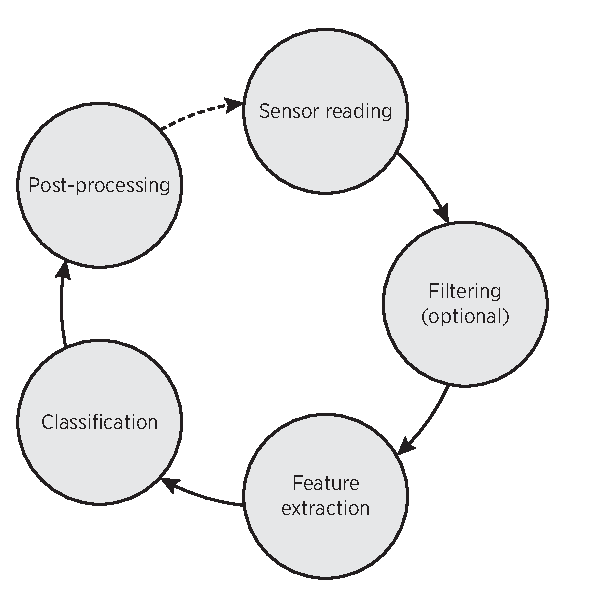
\includegraphics[scale=0.6]{msa-stages}
\caption[Common stages of mobile sensing apps]{Common stages of mobile sensing apps.}
\label{fig-mobile-sensing-apps-stages}
\end{figure}

\subsubsection{Sensing scale of mobile sensing apps}\label{sub:sensing-scale-of-msa}

Depending on the purpose of the mobile app, it may be required to obtain data from one or more users.
The target audience size of the mobile app is known as the \emph{sensing scale}.
There are two sensing scales:
\begin{itemize}
  \item \textbf{Individual sensing scale:} Involves collecting and analyzing data coming from a single person.
  Typically, data refer to track user’s exercise routine and the information is not shared.

  \item \textbf{Community sensing scale:} Involves collecting and analyzing data coming from several users who share a common goal.
  It needs to respond to user specific needs of privacy and anonymity.
  
  This sensing scale is often referred as mobile crowd-sensing and classic examples include traffic monitoring, detection of available parking slots, etc.

  An implicit detail in this sensing scale is the need of a centralized node that acts as a sink of data where analysis processes are executed.
\end{itemize}

This research is conducted targeting the individual sensing scale since the policies to be generated consider analysis of data coming from a single person.


\subsubsection{Paradigms of mobile sensing apps}\label{sub:paradigms-of-msa}

The way how sensors are employed and whether explicit user input is required by a mobile app is known as the \emph{mobile sensing paradigm} \cite{Lane2010}.

There are two sensing paradigms:
\begin{itemize}
  \item \textbf{Opportunistic:} It aims automatic data collection without human participation at all. A remarkable issue of this paradigm is determining the best moment to perform a sensor reading.

  \item \textbf{Participatory:} It leverages the abilities of people requiring their participation to describe the data and to decide the best moment for their capture.

  However, this human dependence can also be a source of errors and noisy data since user is able to upload mislabeled data or even to not to have participation at all.
\end{itemize}


This research is conducted by following the opportunistic paradigm since the smart policies to be generated will decide the duty cycle that sensors must observe, avoiding user participation.


\subsection{Mobile sensing apps examples}
\label{sub:mobile_sensing_apps_examples}

Mobile sensing apps have evolved from apps with specific sensor usage, like using the accelerometer to change the orientation of the screen, to more complex tasks like detecting the user activity e. g. walking, running, climbing stairs, etc.
The usage possibilities offered by mobile sensing apps are high and even increasing after a new sensor is embedded in a smartphone.

In \cite{Wang2012} the \emph{WalkSafe} mobile app is described.
This app improves the safety of pedestrians that walk and talk. WalkSafe leverages the user's context employing the back camera of the smartphone to detect vehicles approaching the user, alerting her or him of a potential unsafe situation.

WalkSafe implements machine learning techniques for detecting the front and back views of moving vehicles.
It employs image recognition algorithms trained off-line with datasets of positive (pictures of front and back views of vehicles) and negative (pictures of side views of vehicles and urban environments) samples producing a set of features for building the car detection model.

Once the model is created, it is uploaded to the phone for its usage in the on-line detection process.
When a phone call is received, the smartphone takes pictures from the back camera, fixes their orientation with accelerometer data, and passed them to the detection module for their processing in real time.
If a car approaching the user is detected, then a vibrating alert is emitted.


Another example of context information usage is \emph{BeWell} \cite{Lane2011a}, which is an app that can monitor and promote some aspects of physical and emotional well-being.
BeWell continuously tracks user behavior along three health dimensions in an \emph{opportunistic} sensing way.

Classifications algorithms are run directly on the phone to infer context information about user's sleep duration, physical activity, and social interaction from sensor data.
BeWell assigns a score to these dimensions and gives a graphical feedback of them to the user.
Sleep duration is inferred by detecting the absence of movement of phone at night.
Physical activity is detected thanks to accelerometer inferring walking, stationary, or running states of the user.
Social interaction is obtained thanks to microphone samples that are used to detect speech or silence time lapses.


A final instance of mobile sensing apps, that employs a \emph{pluggable} sensor via Bluetooth, is \emph{NeuroPhone} \cite{Campbell2010}.
This app works employing neural signals obtained from an electroencephalography (EEG) headset to control smartphones.


Neurophone is a brain-controlled address book dialing app that leverages the generation of P300 \footnote{\emph{P300} is a neuroscience term that refers to a positive peak with a latency of 300 $ms$ that is elicited when brain concentrates on a task specific stimulus among a pool of stimulus.} signals in human brain.
The smartphone shows a sequence of pictures of address book contacts and a potential P300 brain is elicited when a photo matches the person whom the user wishes to call.
The data generated by the EEG headset is transmitted to the smartphone, on which a classification process detects an actual P300 and triggers the contact’s phone number dialing.

% \subsubsection{Convergence of sensing applications into the IoT}
% % Mention that smart devices are connecting people, globally and that is the final objective of them.
% Mobile sensing apps are contributing to the adoption of mobile devices by society.
% By leveraging the communication facilities (for instance, the Internet enabled feature) of smart devices, the vision of future world is one such people will be globally connected with others anywhere and anytime.

% % Mention that a fully connected world has been spotted in other scenarios.
% This vision of a fully connected world has been also chased in other scenarios, like the industry, where the items to be connected are common real world objects like tools, machines, buildings, vehicles, etc.
% % Introduce the smart objects
% Such items are enhanced with an identification mechanism like RFID and basic computation, sensing, and communication facilities that turn them into smart objects \cite{Kortuem2010}.
% % Mention that when 2+ smart objects communicate, then there is a M2M
% Thanks to these enhanced capabilities, the smart objects are able to collect data of their environment and interact with other smart objects, creating a M2M communication system.

% % Introduce the objectives of M2M
% M2M communication systems aim to go beyond the industrial environment and be the base mechanism to query and deliver data between any objects of the real world.
% Such communication should be allowed in any direction, from object A to object B and vice versa.
% Thanks to this, it will be possible to collect data from sensors of a smart object or to instruct an object to behave in a particular way, modifying its environment.

% % Mention that the sets SP-MSA and SO-M2M are similar but also present differences.
% The sets conformed by smartphone--mobile sensing apps and smart objects--M2M target different scenarios but share several features shown in Table \ref{tbl:msa-vs-m2m}.
% The only aspects they do not share are the \emph{communicates with} and application purpose.
% \emph{Communicates with} refers to the type of entity a smartphone or a smart object establish communication with.
% Typically a smart object will communicate always with other smart objects, like in any M2M communication system instance.
% On the other hand, a smartphone can communicate with other objects but also with humans.
% It means that smart devices, like the smartphone, offer several interaction ways for communicating with people while smart objects do not.

% The application purpose marks another difference between smartphones and smart objects.
% A smart object has a specific purpose: it only performs a single or a reduced set of tasks, it is not designed to execute third party apps; indeed, the concept of a mobile OS is out of its scope.
% In change, a smartphone is a general purpose item that can be employed in a wide range of applications. Smart devices include a mobile OS that makes it possible to install third party apps and expand their functionality.
% Broadly speaking, a smart device, like a smartphone, can be considered a smart object but this relationship does not apply inversely.

% \begin{table}
%   \centering
%     \scriptsize
%     \begin{tabularx}{0.70\linewidth}{ccc}
%       \toprule
%       \textbf{Feature} & \textbf{Smartphone} & \textbf{Smart object} \tabularnewline
%       \midrule
%         \textbf{Context awareness} & Yes (Through sensors) & Yes (Through sensors) \tabularnewline
%         \textbf{Communication} & Yes (Wireless) & Yes (Wired, Wireless) \tabularnewline
%         \textbf{Processor} & Yes (Multi-core) & Yes (Low power consuming) \tabularnewline
%         \textbf{Storage} & Yes (In the order of Gigabytes) & Yes (reduced size) \tabularnewline
%         \textbf{\emph{Communicates with}} & Human, other objects & Other objects (machines) \tabularnewline
%         \textbf{Purpose} & General & Specific \tabularnewline
%       \bottomrule
%     \end{tabularx}
   
%     \caption{Comparison of the characteristics of smartphones versus smart objects}
%     \label{tbl:msa-vs-m2m}
% \end{table}

% In any case, the sets smartphone--mobile sensing apps and smart objects--M2M can be abstracted as systems that interconnect \emph{things} in an evolved vision of Internet known as the IoT.
% % Tell a brief IoT interaction-flow
% In the IoT every real world object has a virtual representation and can understand its environment and role in a particular activity, trigger special actions when certain events occur and materialize these actions in both physical and virtual worlds \cite{Uckelmann2011}.
% If mobile computing has the dimension of time and place, IoT adds the new dimension of thing (see Figure \ref{fig-iot-dimensions}).
% Summarizing: IoT aims to produce a fully connected world with unlimited application systems that address any real world problem.

% \begin{figure}
% \centering
% 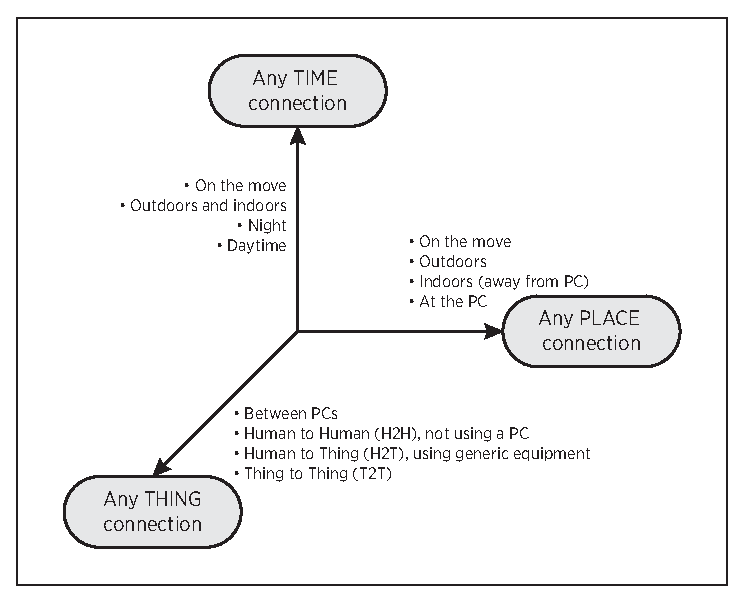
\includegraphics[scale=0.6]{iot-dimensions}
% \caption[Dimensions of the IoT]{Dimensions of the Internet of Things: time, place, thing.}
% \label{fig-iot-dimensions}
% \end{figure}

\section{State of art} 
\label{sec:state_of_art}
This section introduces a description and classification of works aiming to address the energy problem generated by employing sensors continuously in mobile sensing apps.
A special focus is given to the pure software techniques, which will be pursued during the development of this research.

\subsection{Approaches for addressing the energy issue}
\label{sub:approaches_for_addressing_the_energy_issue}

As stated, the advances produced in several technological fields have contributed to the acceptance of the smart devices, like the smartphone, by society \cite{Lane2010,Ra2012}.
However, although computing and storage capacity issues have been partially addressed and solved with every new generation of mobile devices, the energy consumption is still an open issue because of the slow rhythm in technological advances in batteries and because of the inclusion of newer and more sophisticated sensors that impose a higher energy demand.

In this sense, the battery consumption concern has been under research since the introduction of mobile devices into the market, and also shows an evolution in the objectives pursued by scientists. 

The research in energy management in mobile devices started with broad techniques and guidelines applied when building mobile application systems.
In \cite{Mayo2003} the authors address the energy consumption issue from a design point of view by introducing the idea of the \emph{requirements-aware energy scale-down} approach. 

This approach states that both hardware and software elements should scale their features and energy usage to meet a variety of design points.
According to it, if there are no hard energy constraints, the software can use the hardware components at maximum performance in order to accomplish the mobile app requirements.
On the other hand, in case of energy constraints the mobile app must be aware and react accordingly by modifying --- via software --- the hardware usage for consuming less energy and still accomplish the application requirements.
The described work was implemented targeting different hardware elements like screen, processor and wireless radio communication interfaces.
For example, the screen implementation aims the design of energy aware GUI's.
Such GUI's change the luminescence and color of non-active portions of the screen to reduce power consumption, as shown in the Figure \ref{fig-scaling-down-screen-usage}.

\begin{figure}
        \centering
        \begin{subfigure}[b]{0.3\textwidth}
                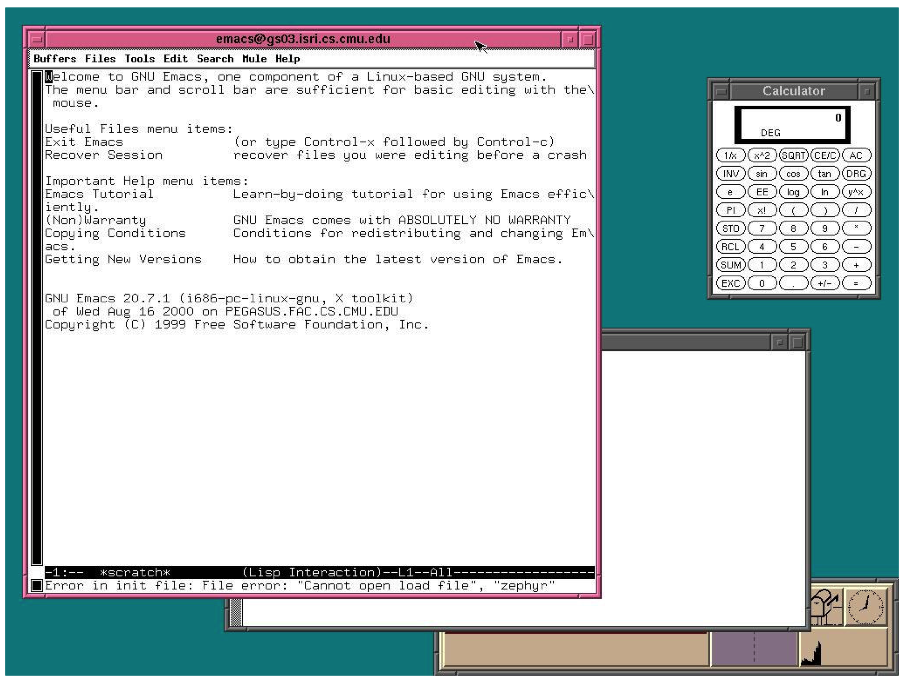
\includegraphics[width=\textwidth]{energy-aware-gui-1}
                \caption{Original interface}
                \label{fig:energy-aware-gui-1}
        \end{subfigure}
        ~
        \begin{subfigure}[b]{0.3\textwidth}
                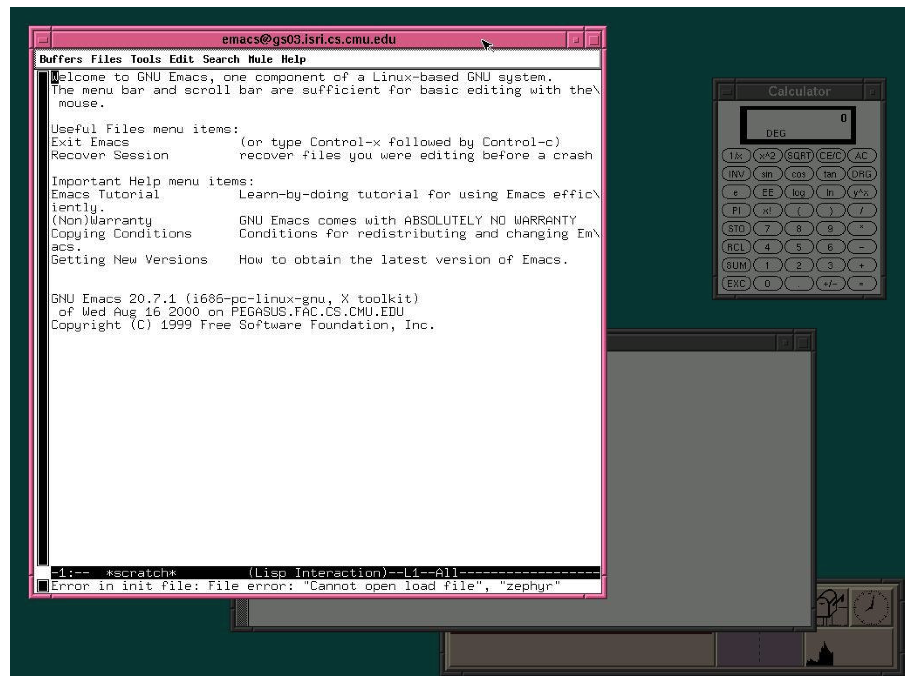
\includegraphics[width=\textwidth]{energy-aware-gui-2}
                \caption{Background half dim}
                \label{fig:energy-aware-gui-2}
        \end{subfigure}
        ~
        \begin{subfigure}[b]{0.3\textwidth}
                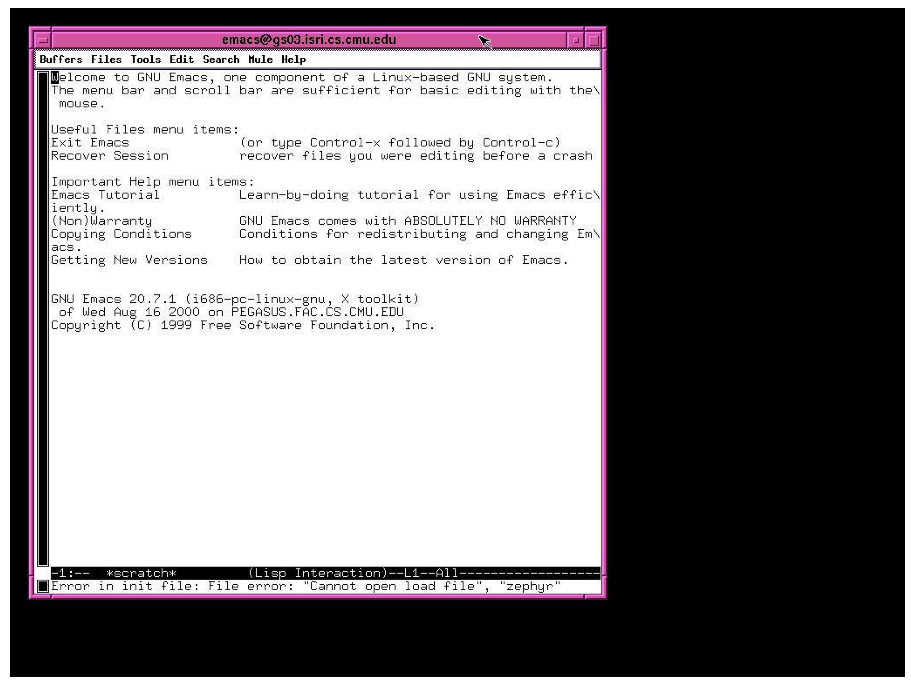
\includegraphics[width=\textwidth]{energy-aware-gui-3}
                \caption{Background fully dim}
                \label{fig:energy-aware-gui-3}
        \end{subfigure}
        \caption[An example of energy aware GUI by \protect\cite{Mayo2003}]{An example of energy aware GUI proposed by \protect\cite{Mayo2003}}
        \label{fig-scaling-down-screen-usage}
\end{figure}

The idea of \emph{requirements-aware energy scale-down} approach serves as a base for the creation of specific techniques for addressing the energy consumption issue.
However, the work introduced by authors focused on broad guidelines that, while helpful, left behind important details that can be obtained from contextual information of user.
It is noteworthy that at the time of the coinage of this approach the smart devices proliferation was in its infancy.

Currently, the popularity of smartphones and the mobile sensing apps have made the energy issue evident and specific mechanisms have been proposed to address it.
A revision of the literature shows that brooadly previous works can be categorized into are three families of techniques to face the energy issue (Figure \ref{fig:approaches-taxonomy}): 

\begin{itemize}
  \item Pure hardware.
  \item Hardware-software.
  \item Pure software.
\end{itemize}

The pure-hardware approach is located at hardware level and is agnostic of the entire software platform.
The hardware-software approach is located at the lowest levels of the mobile OS in connection with hardware elements.
It can be seen as the development of new hardware drivers.
Finally, the pure-software approach is located at top of the mobile OS stack and it is agnostic of the hardware platform.
Works under this approach make use of the API offered by the mobile OS for accessing sensors, collect data, analyze these data and readapt the usage of sensors.

\begin{figure}
\centering
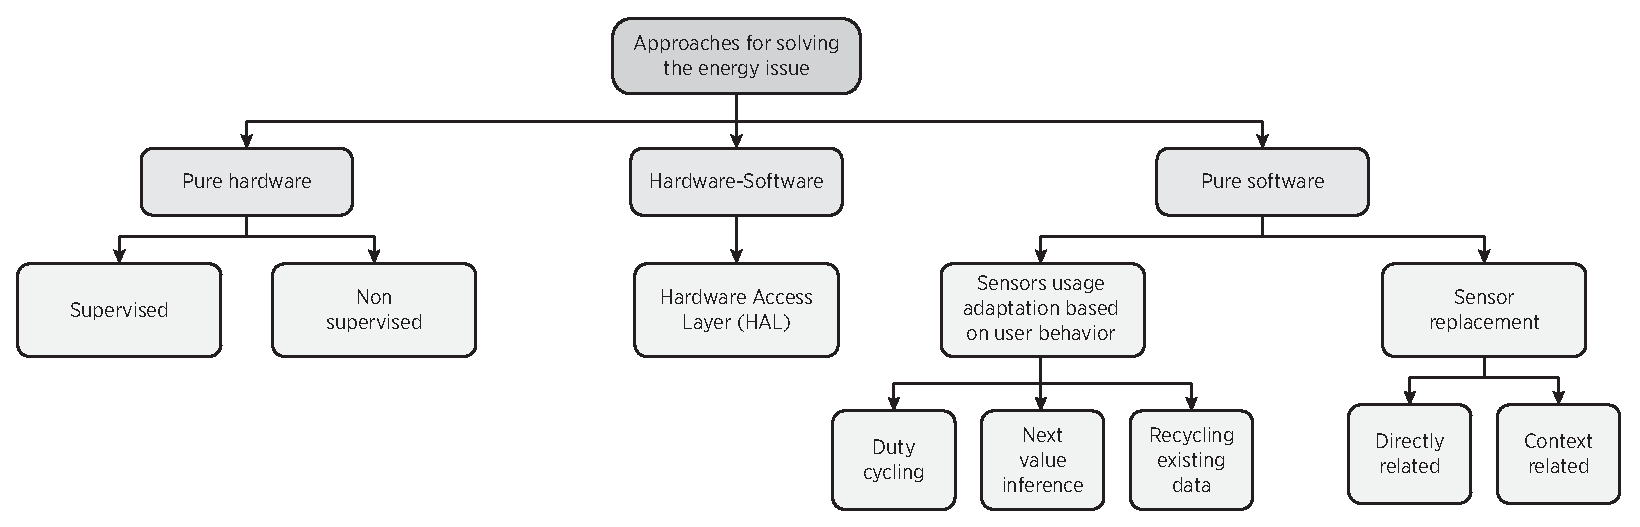
\includegraphics[width=\textwidth]{approaches-taxonomy}
\caption[Taxonomy of approaches for solving the energy issue]{Taxonomy of approaches for solving the energy issue.}
\label{fig:approaches-taxonomy}
\end{figure}

As can be seen in Figure \ref{fig:cross-layer-approaches}, the energy issue is a cross-layer problem that can be analyzed and addressed from several perspectives.
It is noteworthy that although there is a taxonomy of approaches, the solutions found in literature may include a combination of these techniques.
This is a suggestion of the complexity of the problem and even about the evolution of the techniques, since ideas proved to be working efficiently in software soon or later are implemented directly in hardware. 
\begin{figure}
\centering
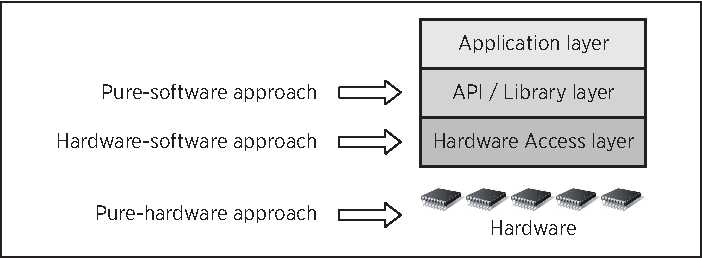
\includegraphics[scale=0.7]{cross-layer-approaches}
\caption[Energy issue as an OS cross-platform problem]{The relation between approaches for solving the energy issue and layers of a mobile platform.}
\label{fig:cross-layer-approaches}
\end{figure}

The Figure \ref{fig:approaches-description} shows the implementation of the three approaches seen from the perspective of the hardware platform.
It is interesting to note that the scope of the pure hardware approach is limited to the adaptation of the different physical variables introduced to the hardware components.
The adaptation of these variables, for example voltage and frequency illustrated in the figure, allows the definition of the power states of the different components, like the idle, active and other statuses.


The same Figure \ref{fig:approaches-description} also allows to detect the main purpose of the hardware – software approach, which is to define periods to keep sensors turned on or off, building a \emph{hardware access layer} above the bolts and nuts of the hardware platform.
Note in the Figure that the usage of the sensor is dictated by a square signal. When this signal has a high value, it turns the sensor on, whereas when it has a low value turns the sensor off. 
The generation of the square signal in this approach is typically done by lower layers of the mobile platform or even by a basic mobile app.


Finally, this Figure \ref{fig:approaches-description} shows the scope of the pure software approach.
Note that in this case, there is also a square signal involved in the behavior of the platform, but instead of controlling just a single sensor it is manipulating several of them.
The generation of this square signal is provided by the smartness present in the mobile app.
Only by leveraging context information it is possible to instruct this complex management of sensors.

% The Figure \ref{fig:approaches-description} shows how the different approaches are implemented in a hardware platform. Note that the pure hardware approach modifies directly the frequency and voltage introduced to the hardware circuits, defining the power states of the components.

% In the same figure, it can be seen that the hardware-software approach defines periods to keep the same sensor turned on or off, building a \emph{hardware access layer} above the bolts and nuts of the platform.

% Finally, the same figure shows that the pure software approach tries to define an even higher layer for modifying the behavior of the different sensors present in the mobile platform. The duty cycling of different sensors can be manipulated in order to obtain high level information --- meaningful for user --- and at the same time lowering the impact on battery.

The Table \ref{tbl:state-of-art-works} shows a set of works found in the literature that aim to solve the energy issue in mobile sensing apps.
An important aspect of these works is that due to their differences in approaches and purpose, it is not possible to perform a direct comparison of them \cite{Vallina-Rodriguez2013}.
The columns considered in the table refers to:
\begin{itemize}
  \item The authors and year of publication of the work.
  \item The approach followed by the work, including the specific variants implemented.
  \item The sensors employed in the work.
  \item The machine learning techniques employed in the work.
  \item The mobile platform where the work was implemented or simulated.
\end{itemize}
Such columns allow to identify the main characteristics present in these works.


{
\scriptsize
\begin{tabularx}{1.0\linewidth}%
  {
  >{\setlength{\hsize}{.6\hsize}\centering\arraybackslash}X
  >{\setlength{\hsize}{.6\hsize}\centering\arraybackslash}X
  >{\setlength{\hsize}{.5\hsize}\centering\arraybackslash}X
  >{\setlength{\hsize}{.8\hsize}\centering\arraybackslash}X
  >{\setlength{\hsize}{.6\hsize}\centering\arraybackslash}X
  }
  \caption{State of art works aiming to address the energy issue in MSA}\tabularnewline
  \toprule
  \textbf{Work} & \textbf{Approach} & \textbf{Sensors involved} & \textbf{Machine Learning Technique} & \textbf{Platform implementation}\tabularnewline
  \midrule
  \endfirsthead

  \toprule
  \textbf{Work} & \textbf{Approach} & \textbf{Sensors involved} & \textbf{Machine Learning Technique} & \textbf{Platform implementation}\tabularnewline
  \midrule
  \endhead

  \midrule
  \multicolumn{5}{c}{\emph{Continue in next page}}\tabularnewline
  \bottomrule
  \endfoot

  %\midrule
  %F1 & F2 & F3 & F4 & F5\\
  %\tabularnewline
  \bottomrule
  \tabularnewline
  \caption{State of art works aiming to address the energy issue in MSA \label{tbl:state-of-art-works}}
  \endlastfoot
  
  \cite{Constandache2009} &
      PS - Sensor usage based on behavior: NVI, DC &
      GPS, Wi-Fi interface, GSM network &
      Custom heuristic with Linear prediction &
      Data collection using Symbian on Nokia N95 phone. Experiments simulated.
      \tabularnewline
      \cmidrule(r){1-5}

      \cite{Kjaergaard2009} &
      PS - a) Sensor usage based on behavior: DC. \newline b) Sensor replacement: DR. &
      GPS, accelerometer &
      Dynamic programming &
      Symbian on Nokia N95 with Python scripts
      \tabularnewline
      \cmidrule(r){1-5}

      \cite{Zhuang2010} &
      HS - HAL &
      GPS, accelerometer &
      Simple decision rule &
      Android 1.5 on G1 Android Development Phone
      \tabularnewline
      \cmidrule(r){1-5}

      \cite{Perez2010} &
      PS - Sensor usage based on behavior: DC &
      GPS &
      Simple decision rule &
      Simulation
      \tabularnewline
      \cmidrule(r){1-5}

      \cite{Lin2010} &
      PS - a) Sensor usage based on behavior: DC, NVI. \newline b) Sensor replacement: DR. &
      GPS, Wi-Fi interface, Bluetooth, Cell tower data &
      Hidden Markov Models and a Bayesian estimation framework &
      Both emulation using datasets obtained from Microsoft and apps running on Android G1 smartphone.
      \tabularnewline
      \cmidrule(r){1-5}

      \cite{Lu2010} &
      PS - Sensor usage based on behavior: DC &
      Accelerometer, GPS, microphone &
      Decision Tree, Markov Decision Process and Gaussian Mixture Models &
      Nokia N95, Apple iPhone
      \tabularnewline
      \cmidrule(r){1-5}

      \cite{Priyantha2011} &
      PH - NA &
      Accelerometer, compass, gyroscope &
      None &
      Custom Hardware on unspecified smartphone phone
      \tabularnewline
      \cmidrule(r){1-5}

      \cite{Perez-Torres2012} &
      PS - Sensor usage based on behavior: DC &
      GPS &
      Simple decision rule &
      Android 2.3.3 on Samsung Galaxy S phone
      \tabularnewline
      \cmidrule(r){1-5}

      \cite{Srinivasan2012} &
      PS - Sensor usage based on behavior: DC &
      Accelerometer &
      Decision Tree &
      Tizen OS on Samsung Galaxy II phone and Android on Nexus S phone.
      \tabularnewline
      \cmidrule(r){1-5}

      \cite{Apple2015} &
      PH - A &
      Accelerometer, compass, gyroscope &
      Not available &
      iOS 8 in iPhone 5s or newer
      \tabularnewline
      \cmidrule(r){1-5}

      \cite{Zhang2013} &
      PS - a) Sensor usage based on behavior: DC. \newline b) Sensor replacement: DR &
      GPS, accelerometer &
      Gaussian Process Regression &
      Android 4.0 on Google Nexus S phone
      \tabularnewline
      \cmidrule(r){1-5}

      \cite{Chon2014} &
      PS - a) Sensor usage based on behavior: DC, NVI, RED. \newline b) Sensor replacement: CR &
      GPS, WiFi interface, Cell tower data &
      Hidden Markov Models &
      Android 2.2 phones.
      \tabularnewline
      \cmidrule(r){1-5}
      
      \cite{Yurur2014} &
      PS - Sensor usage based on behavior: NVI, DC &
      Accelerometer &
      Hidden Markov Models &
      Simulated in Matlab. Implemented on BlackBerry Storm II 9550 phone.
      \tabularnewline
      \cmidrule(r){1-5}

      \cite{Man2014} &
      PS - a) Sensor usage based on behavior: DC. \newline b) Sensor replacement: CR &
      GPS, accelerometer &
      Simple decision rule &
      Android 4.1.4 on Samsung Galaxy SIII i9300 phone
      \tabularnewline
      \cmidrule(r){1-5}

      \cite{Donohoo2014} &
      PS - a) Sensor usage based on behavior: DC. \newline b) Sensor replacement: DR &
      GPS, WiFi network, Cell tower data &
      Linear Discriminant Analysis, Linear Logistic Regression, Neural Network and K - Nearest Neighbor Several &
      Android 2.3.3 phones
      \tabularnewline

  \end{tabularx}
  }

In next sections a brief description of the pure hardware and hardware-software approaches is presented, followed by a detailed review of the pure software approach since the special features and advantages offered by it.
Inside each description some of the works presented in the Table \ref{tbl:state-of-art-works} are also reviewed.

\begin{figure}
\centering
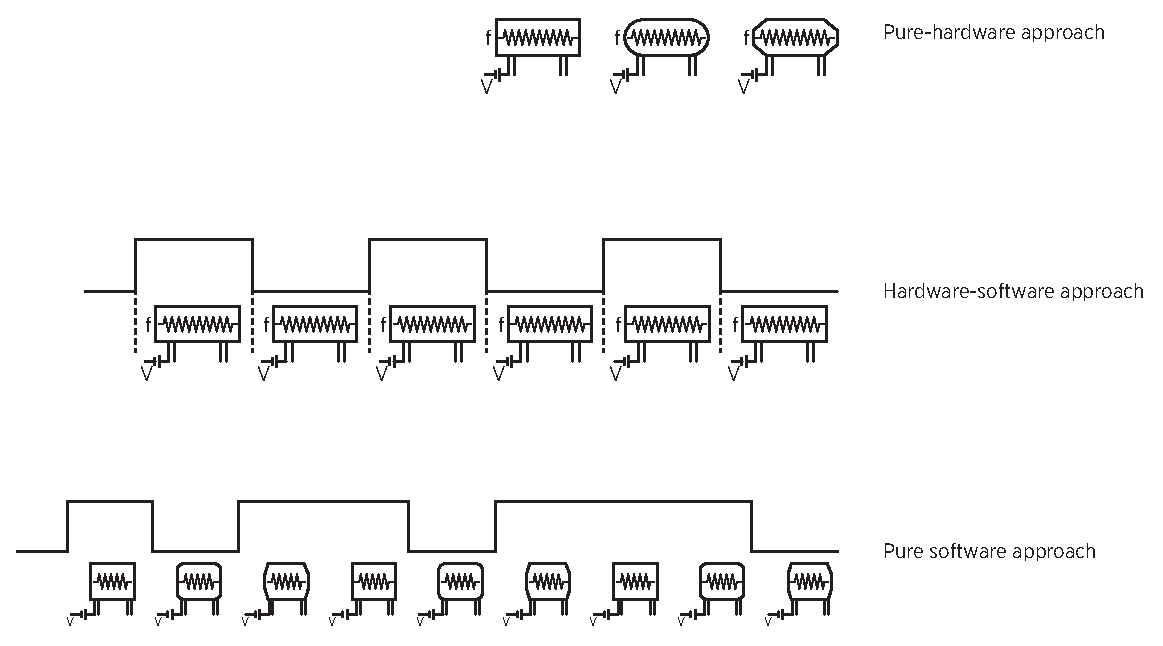
\includegraphics[scale=0.7]{approaches-description}
\caption[Approaches seen from hardware perspective]{The approaches seen from a hardware perspective.}
\label{fig:approaches-description}
\end{figure}

\subsubsection{Pure hardware approach}

Despite the fact current mobile processors include features at the electronic level like DPM\footnote{DPM, Dynamic Power Management} and DVFS\footnote{DVFS, Dynamic Voltage and Frequency Scaling} that are helpful to reduce the energy consumed by them, these techniques are not enough to solve the energy issue in mobile platforms.
The major drawback with the usage of these features is the complexity of the mobile processors, whose static power consumption remains high when the processor is not in sleep mode \cite{Priyantha2011}.
Additionally, the current architecture of most mobile platforms require that for the correct operation of the phone, other components have to be operational, which increases the energy consumption.

This approach is focused in adapting physical features of hardware components in order to reduce the energy consumption.
The most used physical features are the frequency and voltage introduced to the hardware elements.
In this way, the hardware designers define and introduce the different operational states of the physical components of the platform.

Works under this approach typically involve a hardware rearrangement to exploit the previously mentioned features.
This redesign implies the isolation of all of the components associated with the measurement of physical signals inside a new unit with a dedicated low power processor.
Such change must not carry a modification inside the mobile apps' logic.

This new hardware unit can obtain a substantial reduction in the energy consumption since it is energy aware by design.
The basic behavior involves that the sensors report their readings to the embedded low power processor, which is capable of doing light computing operations like filtering.
While the hardware unit is working on reading and filtering data, the rest of the smartphone's hardware platform is able to reach its sleep mode.

%The pure hardware approach can be materialized following two distinct implementations, based on the level of data complexity that the platform can handle.
Depending on the ability to process data and discover contextual information by itself, the pure hardware approach can be implemented in two different ways, namely, the not autonomous and the autonomous variants.

\subparagraph{Not autonomous variant}
\label{subp:not_autonomous_variant}

The \textbf{not autonomous} variant does not have knowledge about the information that is handled and it is restricted to receive sensor data requests and deliver data without running any sort of filtering or processing.

An example of the not autonomous variant is LittleRock \cite{Priyantha2011}.
Its design includes a special unit in charge of the access to sensors.
When any mobile app requires to perform sensing tasks it has the option to employ the LittleRock unit or use it only as a bridge and access directly to sensors.
The relevant features of this design are:

\begin{itemize}
  \item \textbf{Power independence:} LittleRock is powered directly from battery and not from other internal electronic items.
  Because of this, the main circuitry can be turned off when the phone is in sleep mode and keep LittleRock accessing to sensors.
  
  \item \textbf{Interrupt:} LittleRock offers interruption features, making it possible to wake up the phone and inform it about events discovered in data delivered by sensors.
  
  \item \textbf{Re-purposing:} LittleRock allows to reprogram its main processor to adapt the processing of sensor data and achieve mobile app requirements.
\end{itemize}

The experimentation conducted by authors indicates that LittleRock can operate up to 830 days when this and the phone are in sleep mode using a 1340 mAh battery.
Among the results, it is noteworthy that LittleRock is faster than the phone itself do collect a single sample of data from sensors due to the complexity of the software stack that the main processor has to handle.

Another relevant example of the supervised variant is reported in \cite{Choudhury2008}.
Despite the fact this work was not implemented in a smartphone unit, it also introduces a mobile sensing platform (MSP) that is composed in a similar way than LittleRock.
This MSP is basically a sensor board attached to a wireless node that includes a 32 bits ARM7 processor, Bluetooth interface and a compact flash bay for storage.
It can be noted that the MSP is representing the extra hardware unit with sensors and a dedicated low power processor, which can deliver the collected data via Bluetooth to an external computing unit for analysis and classification tasks.


\subparagraph{Autonomous variant}
\label{subp:autonomous_variant}

The \textbf{autonomous variant} is also able to deliver raw data, but additionally can detect higher level information thanks to the data processing algorithms.
For example, it might measure the distance covered by user, the amount of steps done, or identify the type of activity performed by the user (no movement, walking, running, etc.) completely by itself.


The autonomous variant has been already implemented in the Apple iPhone.
Starting from the iPhone 5s model, this smartphones family includes an ARM coprocessor that is in charge of interacting with several sensors like accelerometer, gyroscope and magnetometer in order to obtain data about user's fitness \cite{Sathiah2013}.

Apple has introduced a software API into the iPhone OS, the Core Motion Framework \cite{Apple2015}, that allows mobile app developers to make use of the new hardware architecture and to access and consume this information.
The Core Motion Framework is able to deliver information refering to amount of steps or distance that user has covered and even the type of activity performed by him.
Additionally, this API allows requests for raw data from sensors being the update frequency the only mandatory argument.

Despite the fact this implementation will lead to energy savings, it presents two major drawbacks.
The first one is that the step counter mechanism is always running in the background even if no applications are requesting data.
The second one is that this implementation does not provide support for continuous readings and lacks the idea of self adapting the sensor's duty cycle in order to reduce energy consumption.

A common problem of any hardware approach resides in that hardware designers can not foresee the needs of any future mobile development and implement them directly in the circuits.
In this sense, the effort of hardware designers is affected by a trade off between the features provided out-of-the box and the flexibility features offered by the produced hardware platform.

\subsubsection{Hardware-software approach}

Another approach found in literature describes a combination of hardware and software techniques to optimize the energy consumption in continuous sensing mobile apps.

This approach leverages physical information about sensors and basic data from context information in order to create basic rules to decide the best moment for turning sensors on and off.

% This technique aims to contribute with a reviewed and improved software API that allows to allocate computational and sensing tasks in components others than the predefined by the platform's original design.

By knowing the hardware platform, it is possible to change the behavior of the elements and employ them in a different manner.
An example of this idea is to enable an additional low power processor in the smartphone to execute any arbitrary instruction instead of the main processor.
Since the smartphone's processor can be kept idle there is a potential energy saving.

The work presented in \cite{Ra2012} leverages the presence of several low power processors (LP) in the latest smartphones.
The utilization of these LP's can be done by exposing their functionality through a layered API.

Through several simulations, authors show that such processors can bring substantial energy savings, specially when executing frequent sampling \& buffering and basic arithmetic operations.

That work describes two main challenges, the selection of a suitable LP and guidelines for deciding where to allocate the execution of a given task.
To select an adequate LP, the key factor is the wake up transition delay in terms of energy. So, any processor with a small wakeup transition delay is suitable as LP.
For deciding where to perform the execution of a task, the next guidelines are proposed:
\begin{itemize}
  \item \textbf{Execution in main processor:} {Tasks found to be more efficient in the main processor should be executed there, ignoring the transition penalty}.
  \item \textbf{Execution in LP:} {Tasks found to be more efficient in the LP, and that are very frequent within the mobile app, should be executed in the LP. Sampling and buffering tasks belong to this category}.
  \item \textbf{Execution in main or in LP:}{Tasks found to be more efficient in the LP, and  that are not frequent within the mobile app, should be executed in the LP. However, a special mechanism to evict them should be included. This might happen when tasks of other mobile apps request the LP}.
\end{itemize}


% \begin{table}
%   \centering
%     \scriptsize
%     \begin{tabularx}{1.0\linewidth}{>{\centering}X>{\centering}X>{\centering}X>{\centering}X>{\centering}X}
%       \toprule
%       \textbf{Work} & \centering{\textbf{Approach}} & \centering{\textbf{Sensors involved}} & \centering{\textbf{Machine Learning Technique}} & \centering{\textbf{Platform implementation}}
%       \tabularnewline
%       \midrule
      
%       \cite{Constandache2009} &
%       PS - Sensor usage based on behavior: NVI, DC &
%       GPS, Wi-Fi interface, GSM network &
%       Custom heuristic with Linear prediction &
%       Data collection using Symbian on Nokia N95 phone. Experiments simulated.
%       \tabularnewline
%       \cmidrule(r){1-5}

%       \cite{Kjaergaard2009} &
%       PS - a) Sensor usage based on behavior: DC. \\b) Sensor replacement: DR. &
%       GPS, accelerometer &
%       Dynamic programming &
%       Symbian on Nokia N95 with Python scripts
%       \tabularnewline
%       \cmidrule(r){1-5}

%       \cite{Zhuang2010} &
%       HS - HAL &
%       GPS, accelerometer &
%       Simple decision rule &
%       Android 1.5 on G1 Android Development Phone
%       \tabularnewline
%       \cmidrule(r){1-5}

%       \cite{Perez2010} &
%       PS - Sensor usage based on behavior: DC &
%       GPS &
%       Simple decision rule &
%       Simulation
%       \tabularnewline
%       \cmidrule(r){1-5}

%       \cite{Lin2010} &
%       PS - a) Sensor usage based on behavior: DC, NVI. \\b) Sensor replacement: DR. &
%       GPS, Wi-Fi interface, Bluetooth, Cell tower data &
%       Hidden Markov Models and a Bayesian estimation framework &
%       Both emulation using datasets obtained from Microsoft and apps running on Android G1 smartphone.
%       \tabularnewline
%       \cmidrule(r){1-5}

%       \cite{Lu2010} &
%       PS - Sensor usage based on behavior: DC &
%       Accelerometer, GPS, microphone &
%       Decision Tree, Markov Decision Process and Gaussian Mixture Models &
%       Nokia N95, Apple iPhone
%       \tabularnewline
%       \cmidrule(r){1-5}

%       \cite{Priyantha2011} &
%       PH - NA &
%       Accelerometer, compass, gyroscope &
%       None &
%       Custom Hardware on unspecified smartphone phone
%       \tabularnewline
%       \cmidrule(r){1-5}

%       \cite{Perez-Torres2012} &
%       PS - Sensor usage based on behavior: DC &
%       GPS &
%       Simple decision rule &
%       Android 2.3.3 on Samsung Galaxy S phone
%       \tabularnewline
%       \cmidrule(r){1-5}

%       \cite{Srinivasan2012} &
%       PS - Sensor usage based on behavior: DC &
%       Acceleromete &
%       Decision Tree &
%       Tizen OS on Samsung Galaxy II phone and Android on Nexus S phone.
%       \tabularnewline
%       \cmidrule(r){1-5}

%       \cite{Apple2013} &
%       PH - A &
%       Accelerometer, compass, gyroscope &
%       Not available &
%       iOS 8 in iPhone 5s or newer
%       \tabularnewline
%       \cmidrule(r){1-5}

%       \cite{Zhang2013} &
%       PS - a) Sensor usage based on behavior: DC.\\b) Sensor replacement: DR &
%       GPS, accelerometer &
%       Gaussian Process Regression &
%       Android 4.0 on Google Nexus S phone
%       \tabularnewline
%       \cmidrule(r){1-5}

%       \cite{Chon2014} &
%       PS - a) Sensor usage based on behavior: DC, NVI, RED.\\b) Sensor replacement: CR &
%       GPS, WiFi interface, Cell tower data &
%       Hidden Markov Models &
%       Android 2.2
%       \tabularnewline
%       \cmidrule(r){1-5}
      
%       \cite{Yurur2014} &
%       PS - Sensor usage based on behavior: NVI, DC &
%       Accelerometer &
%       Hidden Markov Models &
%       Simulated in Matlab. Implemented on BlackBerry Storm II 9550 phone.
%       \tabularnewline
%       \cmidrule(r){1-5}

%       \cite{Man2014} &
%       PS - a) Sensor usage based on behavior: DC.\\b) Sensor replacement: CR &
%       GPS, accelerometer &
%       Simple decision rule &
%       Android 4.1.4 on Samsung Galaxy SIII i9300 phone
%       \tabularnewline
%       \cmidrule(r){1-5}

%       \cite{Donohoo2014} &
%       PS - a) Sensor usage based on behavior: DC.\\b) Sensor replacement: DR &
%       GPS, WiFi network, Cell tower data &
%       Linear Discriminant Analysis, Linear Logistic Regression, Neural Network and K - Nearest Neighbor Several &
%       Android 2.3.3 phones
%       \tabularnewline

%       \bottomrule
%     \end{tabularx}
%     \caption{State of art works aiming to address the energy issue in MSA}
%     \label{tbl:state-of-art-works}
% \end{table}


\subsection{The software approach} 
\label{sub:the_software_approach}

The pure software approach focuses in improving the \emph{smartness} level of mobile devices by producing software elements that aid them to obtain a better description about the environment and what the user is doing.

As a result, the smartphone can receive key elements that allow it to have a higher level vision of the user activity and to perform informed decisions to adapt its behavior --- sensor usage --- according to the information discovered from context.
In this sense, human activity understanding is based on the discovery of a pattern in the activity and accurate recognition of the activity itself \cite{Yurur2014a}.

All works under this category aim to collect data from sensors and / or other sources of context, process them to obtain information about user activity and employ this information to direct a smarter usage of sensors and other hardware elements of the smartphone.


\subsubsection{Advantages of the software approach}
The pure software approach offers several advantages over the rest of techniques.
Among these advantages are:
\begin{itemize}
  \item There are millions of smart devices already \emph{deployed} around the word, representing a huge infrastructure ready to be used.
  Modify their hardware and in some cases updating the mobile OS\footnote{OS, Operating System.} itself is almost impossible.
  
  \item Although hardware and hardware-software approaches will lead to an undeniable energy saving, their implementations sometimes is very application specific.
  It is due because of the fact that the isolated sensing unit is only capable for being configured for a single mobile app.
  
  \item Current OS's and SDK's\footnote{SDK, Standard Development Kit, the set of compilers, libraries and additional content that allow a programmer to develop applications for that platform (hardware and software).} make it possible to implement a pure-software approach in a logical software unit, such as a middleware or framework.
  This software unit can be embedded in a mobile app just like any other 3rd party library.
  Moreover, it can be installed standalone in the mobile OS and be consumed by mobile apps, in a similar manner the .NET Framework and the Java runtime are installed and utilized.

  \item  By implementing such cognitive processes in the higher software layers, they can be configured, tuned, packed and distributed for their usage in mobile apps running in millions of mobile devices.
  
\end{itemize}

From these points, the most important one is the opportunity to give a smarter behavior to the smartphone and make it participant of higher logical level activities. In this way, the mobile devices are able to detect what the user is doing and how is he/she doing it. Giving this \emph{smartness} opens the path for doing a directed usage of sensors, resulting in energy savings and the adquisition of proper and relevant information.

Based on research in literature, two main branches of the pure software approach has been identified. These branches are described in the next sections.

\subsubsection{Sensors usage adaptation based on user behavior}
\label{ssub:sensors_usage_adaptation_based_on_user_behavior}

It is based on analyzing processes of historical data for detecting patterns in the user behavior.
Once a pattern is detected it is employed to adapt the usage of the sensors.
The new specifications for the sensors usage depends on the purpose of the mobile app framework, however three decisions has been identified.

\subparagraph{Duty cycling}
\label{subp:duty_cycling}
This specific technique tries to adapt the sensor access frequency to reduce energy consumption.
Because of the existence of sleep periods in the sensor being \emph{duty-cycled}, this technique may introduce energy - precision tradeoffs.

In \cite{Perez-Torres2012} a power aware middleware for the support of location and context aware mobile apps with cloud computing interaction is presented.
This middleware incorporate a simple decision rule for determining whether user is in motion. If motion is detected the the GPS continuous readings increment their frequency, otherwise they decrement it.
Through this basic notion of policy authors identified a tendency to obtain energy savings, incrementing the battery life up to 3 times.

\subparagraph{Next value inference}
\label{subp:next_value_inference}
This technique also relies in analysis processes over historical data in order to obtain an approximate inference of the next value that sensors may deliver.

As can be inferred, an actual access to sensor is avoided which may help to reduce energy consumption.
The energy efficiency of this tehcniques depends on the trade-off between the energy consumption of an actual sensor reading against the energy consumed by the computing processes to obtain its inference. Because of this, such technique is useful only when employing high energy consuming sensor or for its use in distributed systems as shown by \cite{Musolesi2010}

\subparagraph{Recycling existing data}
\label{subp:recycling_exsisting_data}
This technique tries to identify common or frequent circumstances or events in contextual information in order to deliver data generated previously.
In this way, an actual access to sensors is also avoided.

In \cite{Chon2014} an energy efficienct mobility monitoring system, FreeTrack, is presented.
This model employs Hidden Markov Models to model the user location inference by collecting data from sources different than GPS.
In this way, the system can identify the place where the user is, for example, employing data coming from cellular and WiFi networks and even from the battery state.

Despite the advantages offered by FreeTrack, a 68\% of energy savings and a precision of 97\% in daily location traces, the main issue is that the system only gives a semantic idea of place as output (e.g. at home, or at work, etc.) instead of location coordinates. 
Because of that there is no way to perform calculations of distance and mobile applications should only use what the system obtains. 
Additionally, FreeTrack may not work if cellular communication is not available or if the user travels constantly since it will begin to miss places frequently.


\subsubsection{Sensor replacement}
\label{ssub:sensor_replacement}

The sensor replacement branch considers the semantic of data in order to find another source of context information.

It refers to consider the purpose of data reading in order to find a different way to obtain the same information. For example, GPS receiver is employed for obtaining the user location but the cellular network data or the wireless networks may also deliver such class of information; even other values like the time of the day and accelerometer data may suggests the location of user.

It is noteworthy the existence of an implicit energy – precision tradeoff due to the changes in the source of context information.
Depending on the relationship of the sensors, there are two types of replacement:

\subparagraph{Directly related replacement}
\label{subp:directly_related_replacement}
The sensor is replaced with another sensor, less energy consuming, that delivers the same type of data without the need of mapping them or additional processing tasks.

In \cite{Lin2010} the A-Loc (adaptive location provider system) is presented.
Based on the accuracy level required by mobile apps, A-Loc chooses the best medium for obtaining user location among GPS, WiFi, cellular tower triangulation and Bluetooth.
% Qué se le critica aquí a A-Loc.

\subparagraph{Context related replacement}
\label{subp:context_related_replacement}

The sensor is replaced with another one that does not deliver the same type of data.
A special process for translating or mapping data is needed for their usage by mobile apps.

In the previous cited work, FreeTrack \cite{Chon2014}, the battery status is employed to determine user location.
Authors consider that users typically charge their smartphones at very well known places, like home or work.
By checking whether battery is charging, the possibilities for deciding user location are dramatically reduced.

However, since the raw data delivered by the new sensor have to be translated, the energy - precision tradeoff is affected heavily: an error in the mapping may bring serious problems.
In the case of FreeTrack, a user charging the smartphone while driving in car causes to obtain wrong results by the software platform.

\subsubsection{Machine learning techniques employed in literature}

In order to detect information about user's context, the mobile app has to employ specific mechanisms to turn the raw data from sensors into information with a significant meaning to the user.

Because of the complexity of human activities and the noise existing in sensor data, the classification algorithm are almost always probabilistic, although machine learning techniques have also been used \cite{Choudhury2008}.

In \cite{Donohoo2014} a description of the most used machine learning techniques is presented. The description of these techniques is summarized in Figure \ref{fig:ml-techniques}.

\begin{figure}
\centering
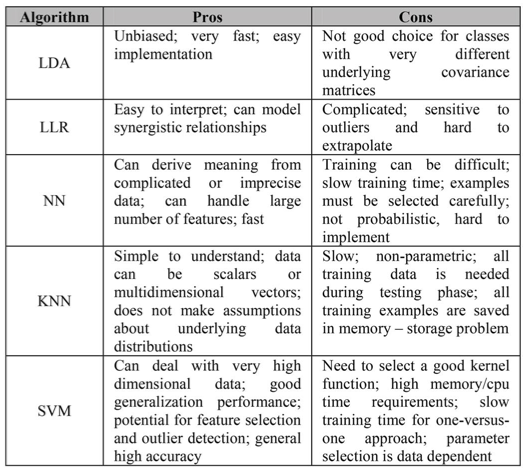
\includegraphics[scale=1.2]{ml-techniques}
\caption[Most used machine learning techniques]{Most used machine learning techniques for modeling user behavior patterns.}
\label{fig:ml-techniques}
\end{figure}

% \begin{itemize}
%   \item Machine learning techniques for determining user behavior

%   \begin{itemize}
%     \item Duty cycling: Adapt the frequenc of use of sensors.
%     \item Next value inference: Infer the next value of the sensor.
%     \item Recycling existing data: From previous information.
%   \end{itemize}

%   \item Sensor replacement: Use less expensive sensors.

%   \item Sensor fusion: Employ different sensors to obtain the data.
%   \begin{itemize}
%     \item Sensors directly related: Several sensors can deliver the same kind of information. For example, location can be obtained via mobile network cell, WiFi and GPS. Use the less expensive sensors.
%     \item Sensors related by contextual information.
%     Even not directly related sensors can be employed to infer the same kind of information. For example, a charging battery, a constant cell ID or static accelerometer data may mean that user is not in motion.
%   \end{itemize}

% \end{itemize}


\section{Proposed method}
\label{sec:proposed_method}

In this stage of the research the basic structure of the method to solve the energy issue in the mobile sensing apps has been defined.
The Figure \ref{fig:methodology-stages} shows the workflow of this method.
However, prior to the description of the method elements, it is important to remark the scope of the current research.

\begin{figure}[h]
\centering
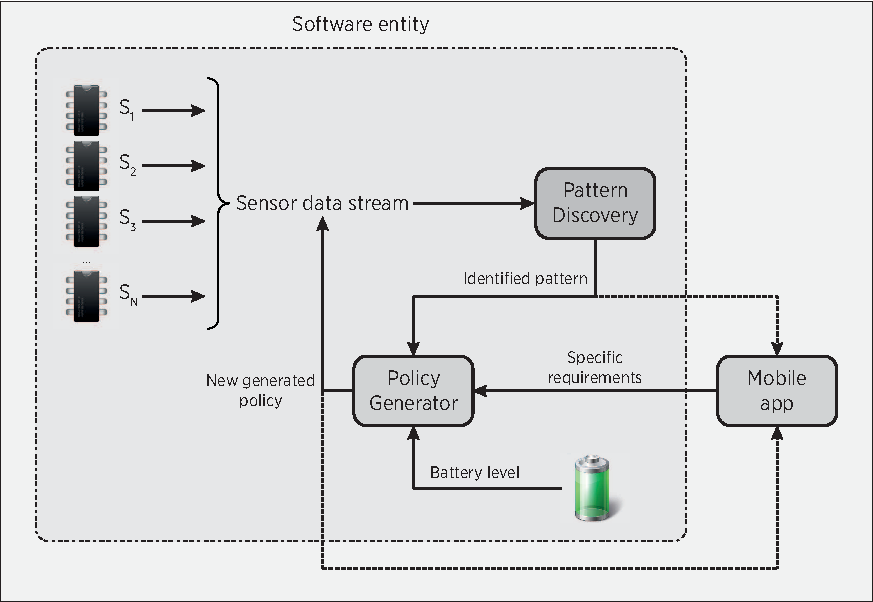
\includegraphics[scale=0.7]{methodology-stages}
\caption[Workflow of the proposed method]{Workflow of the proposed method.}
\label{fig:methodology-stages}
\end{figure}

\subsection{Scope of the research} 
\label{sub:scope_of_the_research}

The work to be performed in this research will be materialized in a software element following:
\begin{itemize}
	\item The pure-software approach.
	\item The individual sensing scale.
	\item The opportunistic paradigm.
\end{itemize}

Additionally, the sensors to be employed are the ones describing motion --- \emph{inertial sensors} --- like GPS and accelerometer, as suggested by the committee in the thesis proposal defence.
The patterns to be identified in data captured from sensors are still to be defined.
Also, these patterns' representation is in process of definition.
However, it is possible to state that a tentative set of patterns can be composed of \emph{no movement}, \emph{walking}, \emph{running}, and \emph{moving in vehicle}.

\subsection{Data acquisition} 
\label{sub:data_acquisition}
As can be seen in Figure \ref{fig:methodology-stages}, the data acquisition is the starting and ending point of the method's workflow.
This component will be in charge of gathering streams of data that will be used later to discover a pattern in user behavior.
It is important to note that this element will be influenced by the feedback information generated by the \emph{Policy generator element}.

\subsection{Pattern identifier element} 
\label{sub:pattern_identifier_element}
This component will receive the sensors data coming from the \emph{Data acquisition} module.
Since this component has to perform data analysis tasks, it should include a memory mechanism for storing and accesing data.
The pattern recognition techniques for identifying relevant events in sensor data are also to be researched, selected and possibly adapted for its execution in a smartphone.

\subsection{Policy generator element} 
\label{sub:policy_generator_element}
This component will create policies based on the pattern identified from sensor data, precision and energy hints provided by mobile app, and current status of physical constraints (battery level) of mobile platform.
Because of this, it is the element that supplies \emph{smartness} to the platform.
The policy created can be implemented by modifying the duty cycling of sensors.

The definition and representation of the policy are also in process of definition.


\section{Conclusions}
\label{sec:conclusions}
Mobile devices, like the smartphones, have become sophisticated computing elements that have the capability of sensing the environment. 
Numerous examples of mobile apps leveraging the sensing and computing features of the smartphones can be found in the market, being known as mobile sensing apps.

The mobile sensing apps expand the benefits that smartphones can offer, but also have a great impact in the energy consumption of the devices.
The energy consumption represent a complex and cross layer issue that has been tried to solve from several perspectives.
This technical report has presented a brief description of this problem, a revision of the basic elements for its comprehension and a taxonomy of the works aiming to solve this issue.

Finally, the revision of a pure software solution for this problem is also described.
This solution aims to increase the smartness level of the mobile platform, becoming aware of the environment for making informed decisions about the sensors usage.


\bibliographystyle{siam}
\bibliography{../../../resources/references/bibliography}

\end{document}
